\section{Results}
\label{sec:four}
\subsection{Regression}
We now present the results for regression and classification task.

In regression, we run cross validation for three methods: baseline, linear regression, and polynomial with degree two for different sets of top-k features. We use MSE to measure the performance. The results are presented in the left graph of Figure~\ref{fig:training}. 

Both linear regression and polynomial regression can easily overcome the baseline. Polynomial regression performs a little bit better than linear regression. The performances become better if we use more features. However, using too many features does not help because of the correlation between them. 

Based on those results, using 10 selected features help linear regression achieve the best result. Meanwhile, 7 selected features are enough for polynomial regression. In practice, we will choose polynomial regression as our final model and report only one result from it. Here, for demonstration purpose, we also run baseline and linear regression with the best setting on testing data. The results are presented in Table~\ref{tab:regperf}.

As we can see, polynomial regression still maintains a good performance compare to linear regression and beats the baseline by a significant amount.

\begin{table}[t]
  \caption{Regression performance comparison of (1) baseline, (2) linear
    regression and (3) polynomial regression of degree two as measured using the
    mean squared error on the test data set.}
  % \centering\small
  % \renewcommand{\tabcolsep}{1pt}
  \newcolumntype{C}{>{\centering\arraybackslash}X}%
  % \newcolumntype{R}{>{\raggedleft\arraybackslash}X}
  \begin{tabularx}{\linewidth}{@{\kern3pt}cCc@{\kern3pt}}
    \toprule
    \bfseries Model & \bfseries Top-$k$ Features & \bfseries MSE \\
    \midrule
    (1) & --- &  12.60835 \\
    (2) &  10 &  0.047144 \\
    (3) &  7  &  0.032311 \\
    \bottomrule
  \end{tabularx}
\label{tab:regperf}
\end{table}

\subsection{Classification}
We continue apply the same procedure in classification task. The right graph in Figure~\ref{fig:training} shows F1-score of baseline, k-NN with k equals 1 and 5, and Random Forest with 10 and 50 trees.

Only random forests with a small number of features can (barely) beat the baseline. Both random forest settings achieve the best result when using 6 features. The performances become worse when the number of features increases. Random forests with 50 trees catches up with the baseline when we used almost all features.

k-NN only overcome the baseline by a very little margin when using 1 or 2 features. Both k-NN settings have the best result with 2 features. The rest perform much worse than the baseline. There is one interesting dip in the performance when using k-NN with 1 neighbor and 3 features.

Our final model we choose is random forest with 50 trees and using 6 best selected features. For demonstration purpose, we train all models with the best settings and run on the test data. The results are presented in the Table~\ref{tab:clsperf}

Our final model still returns the best result on the data set although by not much when comparing to the baseline. Other models surpass the baseline by a small margin as well, except for k-NN with 1 neighbor and 2 features which gives a very low performance.

\begin{table}[t]
  \caption{Classification performance comparison of (1) baseline, $k$-NN with
    (2) 1 and (3) 5 neighbors, random forest with (4) 10 and (5) 50 decision
    trees as measured using the \fmeasure{} on the test data set.}
  % \centering\small
  % \renewcommand{\tabcolsep}{1pt}
  \newcolumntype{C}{>{\centering\arraybackslash}X}%
  % \newcolumntype{R}{>{\raggedleft\arraybackslash}X}
  \begin{tabularx}{\linewidth}{@{\kern3pt}cCc@{\kern3pt}}
    \toprule
    \bfseries Model & \bfseries Top-$k$ Features & \bfseries \fmeasure{} \\
    \midrule
    (1) & --- & 0.771499 \\
    (2) &   2 & 0.024242 \\
    (3) &   2 & 0.782774 \\
    (4) &   6 & 0.813008 \\
    (5) &   6 & 0.813513 \\
    \bottomrule
  \end{tabularx}
\label{tab:clsperf}
\end{table}

\begin{figure*}[h]
\centering
\begin{minipage}{.49\textwidth}
  \centering
  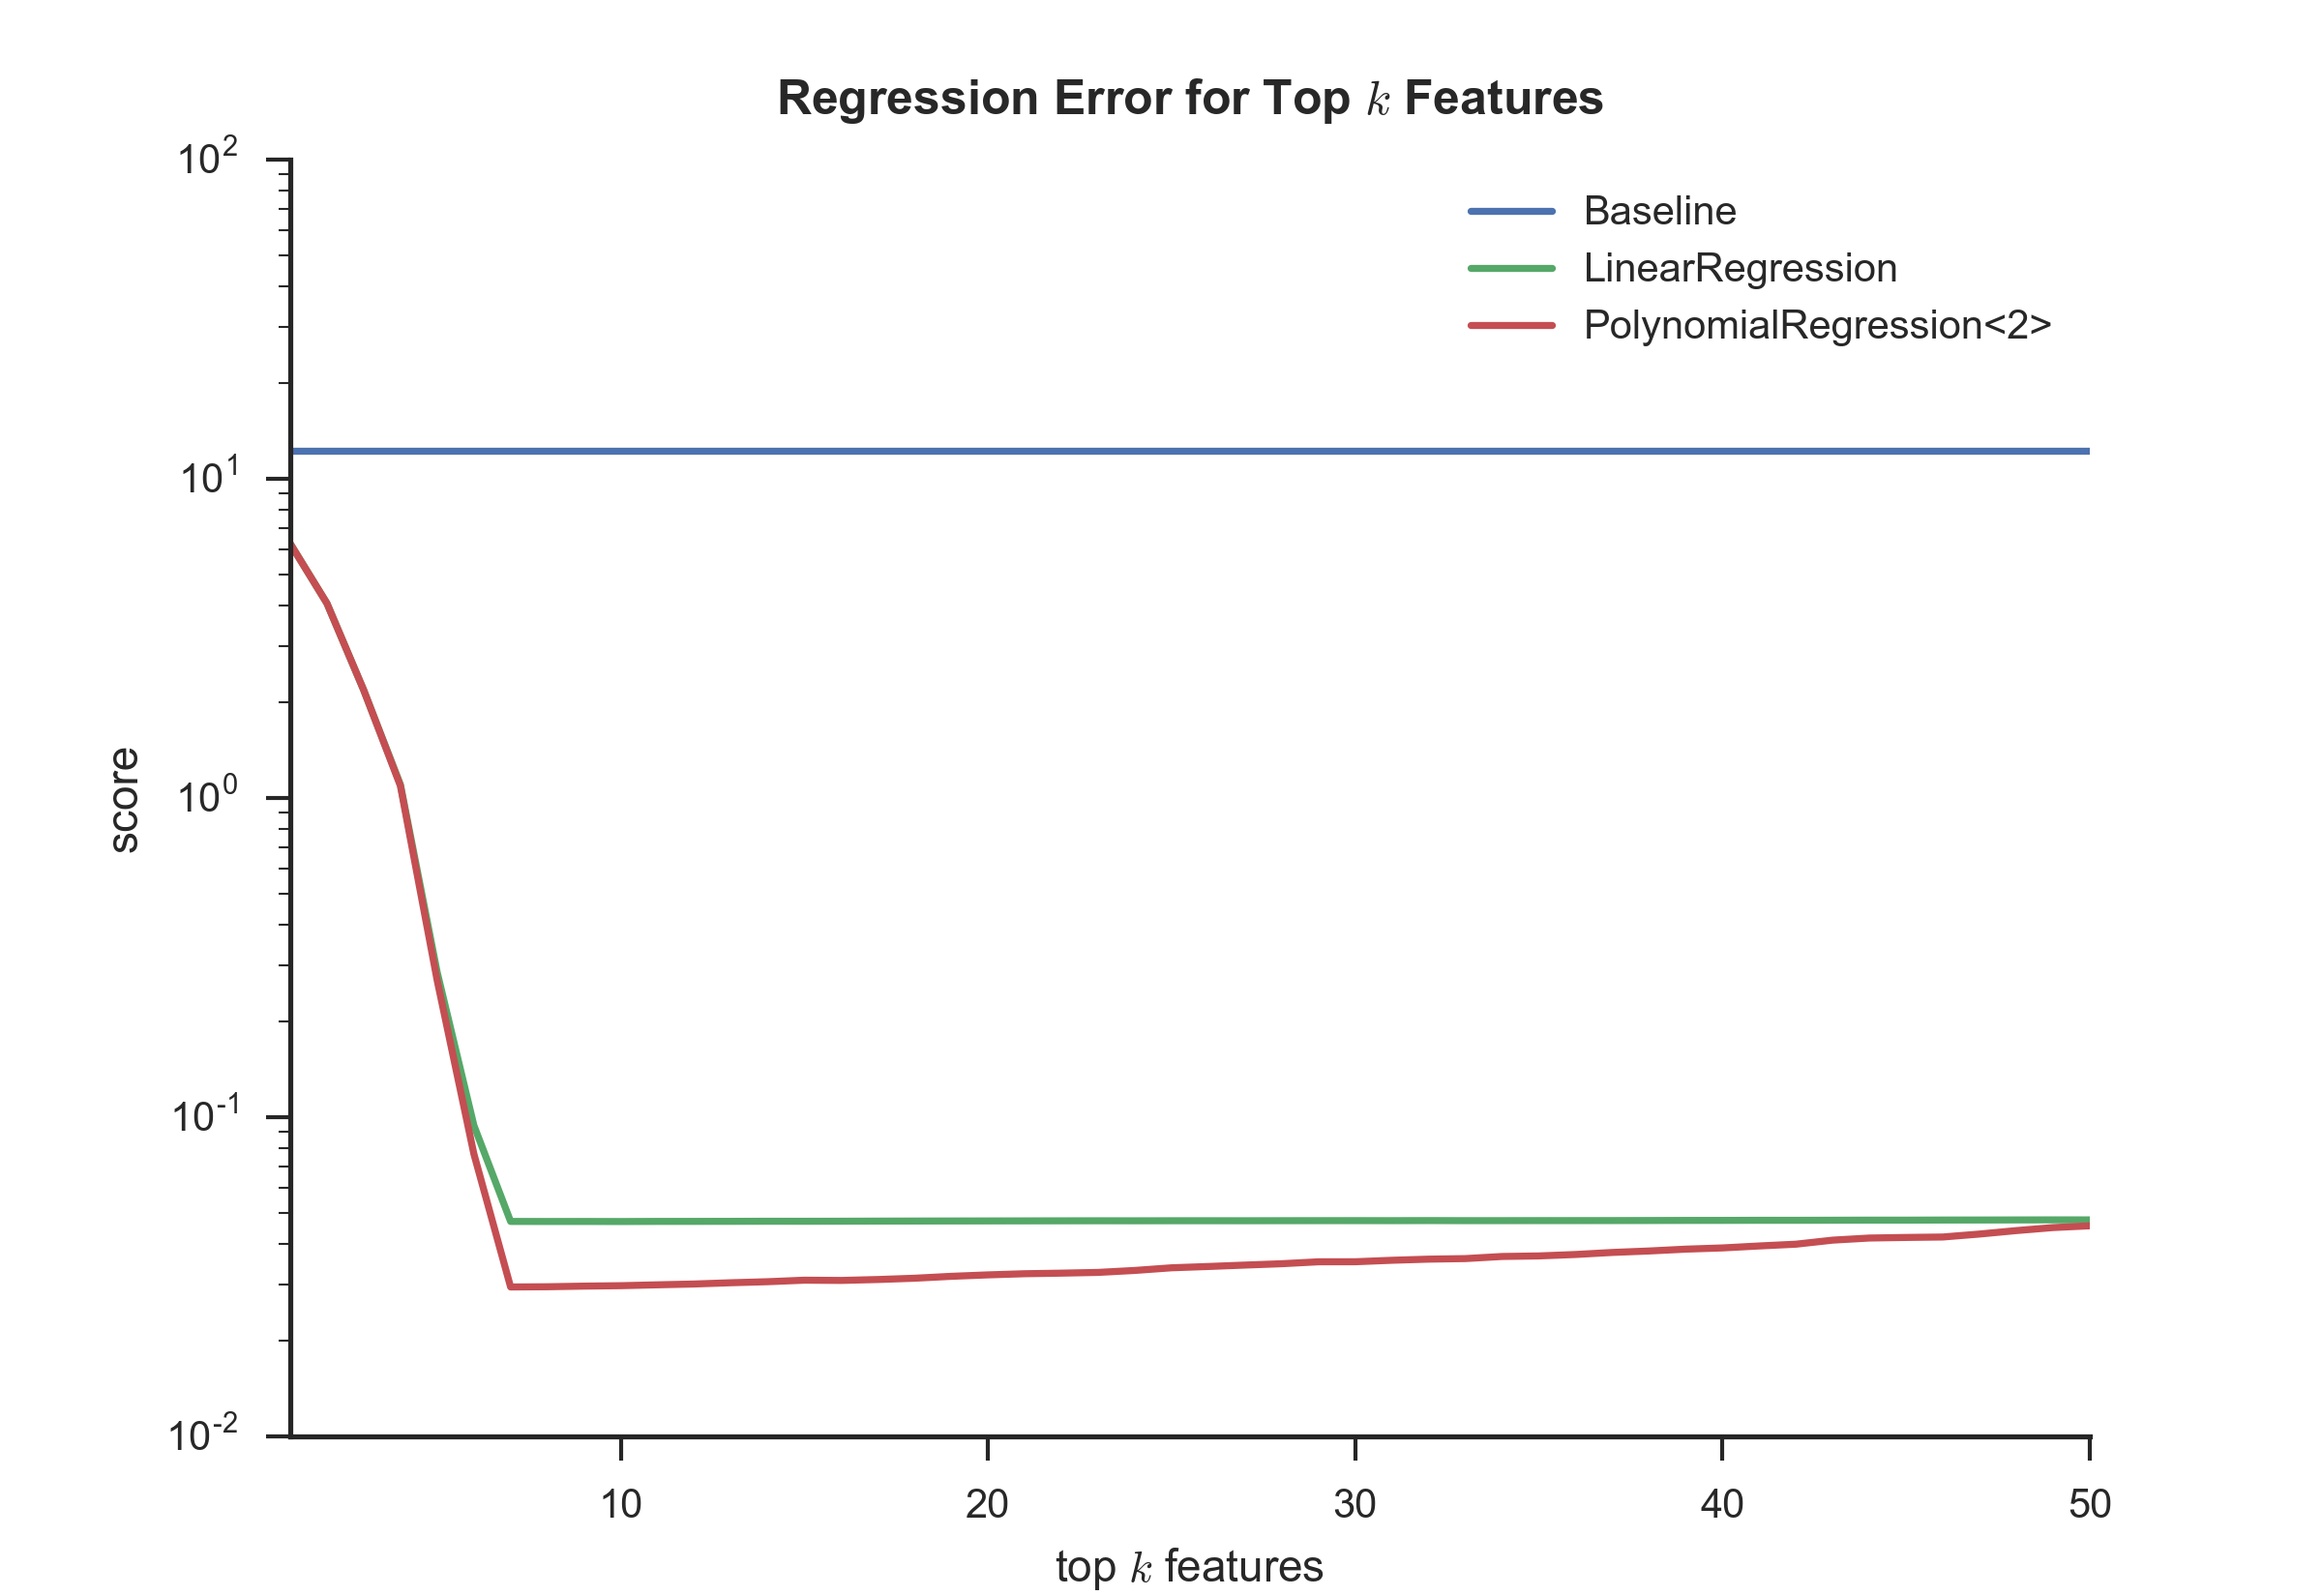
\includegraphics[width=\linewidth]{figures/reg_mse_train.png}
\end{minipage}
\begin{minipage}{.49\textwidth}
  \centering
  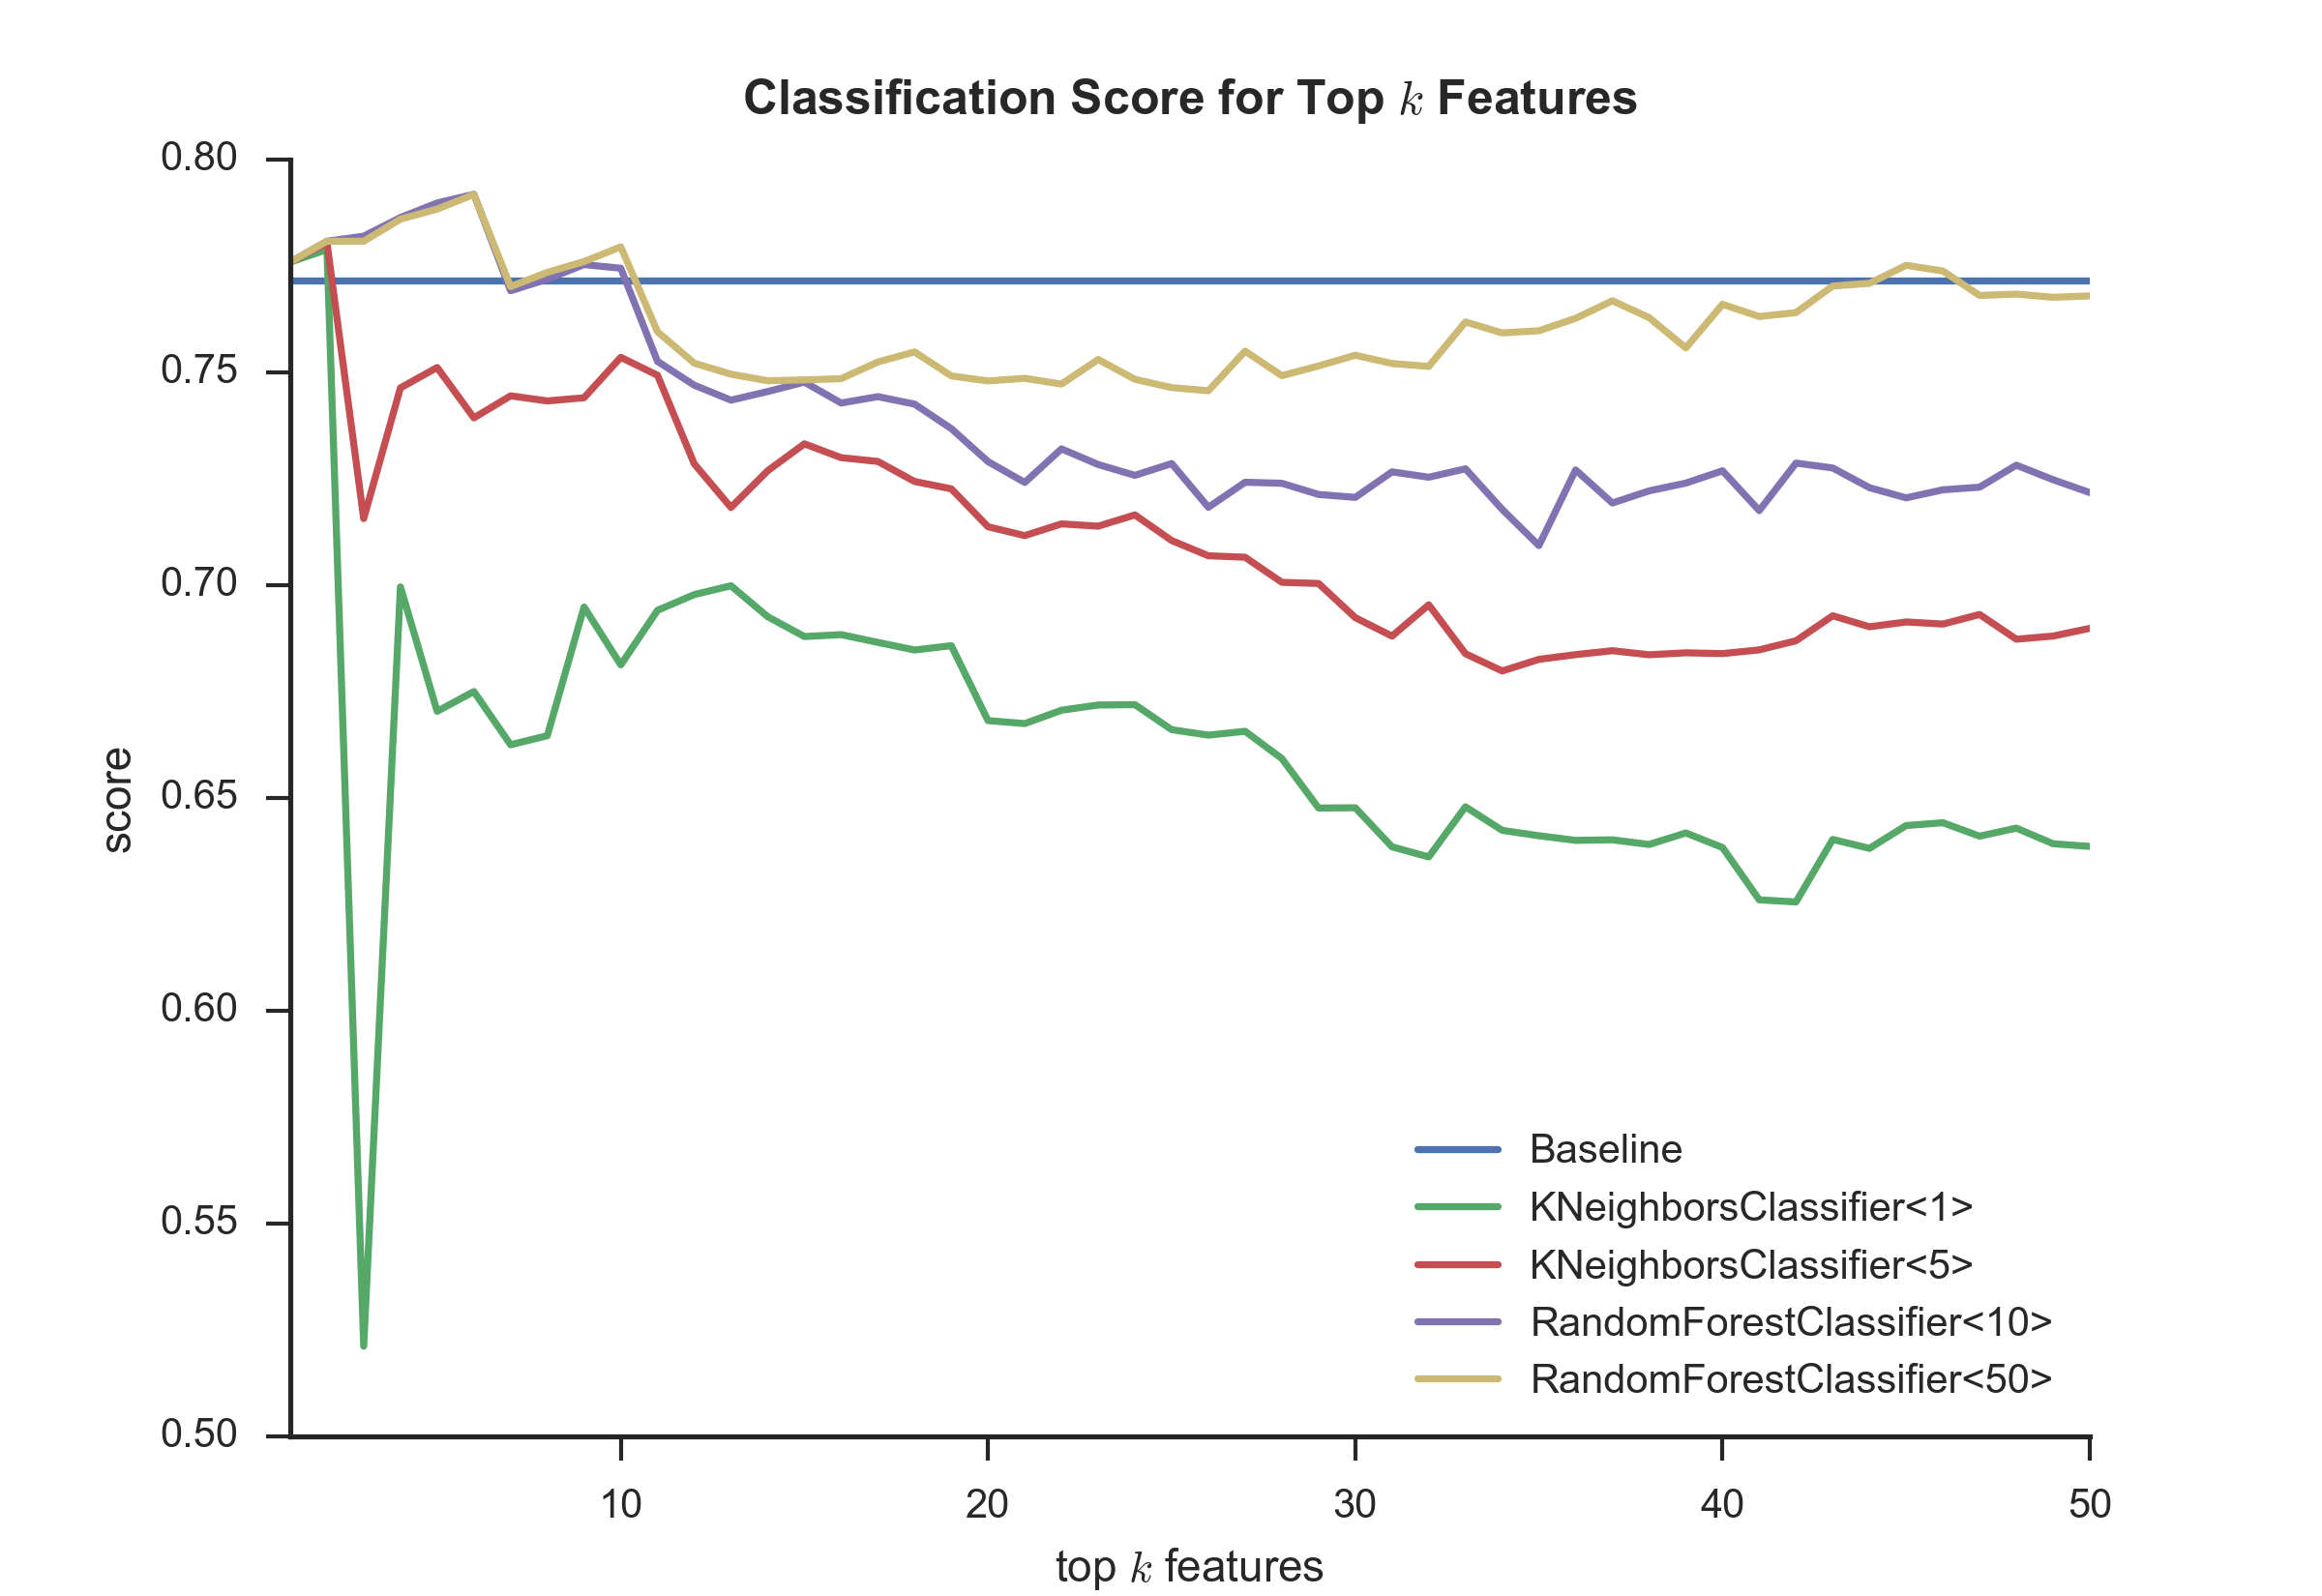
\includegraphics[width=\linewidth]{figures/cls_fscore_train.png}
\end{minipage}
\caption{Performance graphs for regression (left) and classification (right) for
  number of top-$k$ features, evaluated with MSE and \fmeasure, respectively.}
\label{fig:training}
\end{figure*}

%%% Local Variables:
%%% mode: latex
%%% TeX-master: "../main"
%%% End:
